\documentclass[11pt]{article}

\usepackage[margin=1in]{geometry}
\usepackage[T1]{fontenc}
\usepackage[utf8]{inputenc}
\usepackage{lmodern}
\usepackage{amsmath}
\usepackage{booktabs}
\usepackage{xcolor}
\usepackage{hyperref}
\usepackage{tikz}
\usetikzlibrary{arrows.meta,calc,positioning}

\hypersetup{
    colorlinks=true,
    linkcolor=black,
    urlcolor=blue
}

\definecolor{maskcyan}{HTML}{19C6D4}
\definecolor{axispurple}{HTML}{B875FF}
\definecolor{podred}{HTML}{D00000}
\definecolor{helpergray}{HTML}{777777}
\definecolor{psorange}{HTML}{F0A020}
\definecolor{gridgray}{HTML}{D8D8D8}

\title{Pelvic Outlet Diameter Medial Axis Calculation}
\author{2D Point Annotator}
\date{Current application implementation}

\begin{document}
\maketitle

\section*{Purpose}

This note describes how the application now calculates the medial axis used to
construct the pelvic outlet diameter (POD) line. The calculation is performed in
the 512 by 512 manual contour mask space, independent of the displayed image size
or original image resolution. The resulting construction points are converted
back to image coordinates for viewing and for the derived POD line annotation.

\section*{Inputs and Output}

\begin{center}
\begin{tabular}{lll}
\toprule
Input & Required & Role \\
\midrule
\texttt{L-C-PO} & yes & left pelvic outlet contour, drawn on image right \\
\texttt{R-C-PO} & yes & right pelvic outlet contour, drawn on image left \\
\texttt{L-LPO} & yes & derived left lateral pelvic outlet point \\
\texttt{R-LPO} & yes & derived right lateral pelvic outlet point \\
\texttt{L-C-PS} & optional pair & left pubic symphysis contour evidence for the axis \\
\texttt{R-C-PS} & optional pair & right pubic symphysis contour evidence for the axis \\
\bottomrule
\end{tabular}
\end{center}

The output is the derived \texttt{POD} line segment. Its endpoints are selected
on the left and right pelvic outlet contours, but the centerline used to orient
that segment is fit from both the pelvic outlet contours and, when available, the
pubic symphysis contours.

\section*{Coordinate Convention}

Protocol side labels are patient-side labels. On the displayed AP image, the
patient's left side appears on image right, and the patient's right side appears
on image left. Therefore, for this POD calculation:

\begin{itemize}
    \item the medial edge of \texttt{L-C-PO} or \texttt{L-C-PS} is the smallest
    active \(x\) value on a row;
    \item the medial edge of \texttt{R-C-PO} or \texttt{R-C-PS} is the largest
    active \(x\) value on a row.
\end{itemize}

\begin{figure}[htbp]
\centering
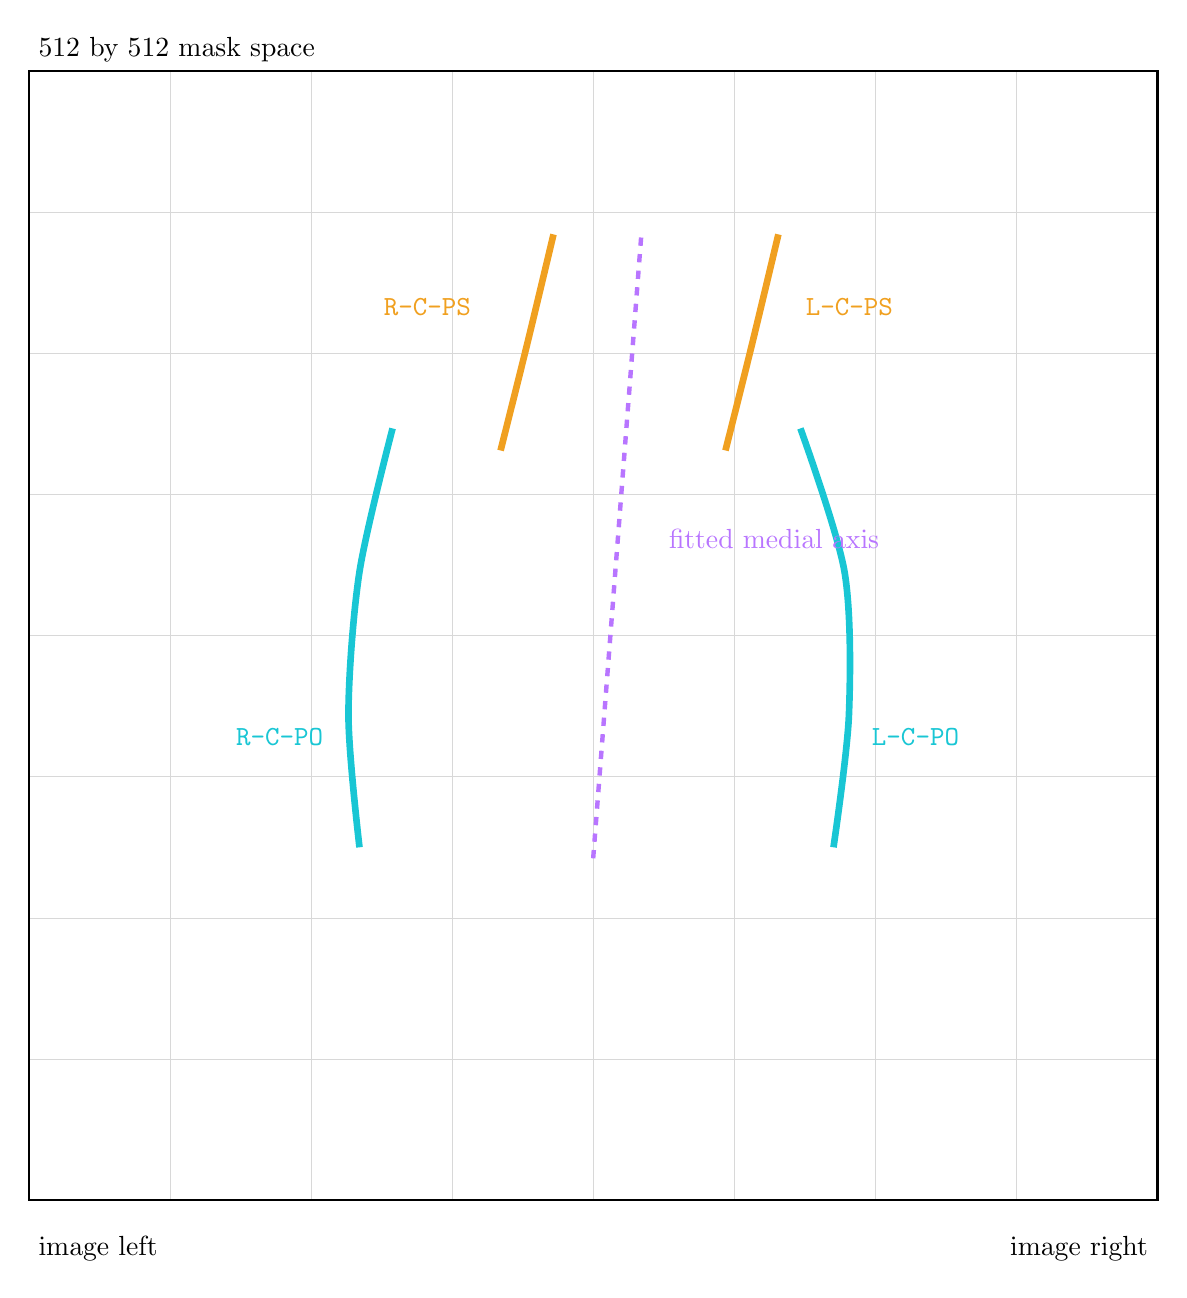
\begin{tikzpicture}[x=0.028cm,y=0.028cm]
    \draw[step=64, gridgray, very thin] (0,0) grid (512,512);
    \draw[black, thick] (0,0) rectangle (512,512);
    \node[anchor=south west] at (0,512) {512 by 512 mask space};
    \node[anchor=north west] at (0,-12) {image left};
    \node[anchor=north east] at (512,-12) {image right};

    \draw[maskcyan, line width=2.4pt] plot[smooth] coordinates
        {(150,160) (145,220) (150,285) (165,350)};
    \draw[maskcyan, line width=2.4pt] plot[smooth] coordinates
        {(365,160) (372,220) (370,285) (350,350)};

    \draw[psorange, line width=2.4pt] plot[smooth] coordinates
        {(214,340) (226,388) (238,438)};
    \draw[psorange, line width=2.4pt] plot[smooth] coordinates
        {(316,340) (328,388) (340,438)};

    \node[maskcyan, anchor=west] at (378,210) {\texttt{L-C-PO}};
    \node[maskcyan, anchor=east] at (138,210) {\texttt{R-C-PO}};
    \node[psorange, anchor=west] at (348,405) {\texttt{L-C-PS}};
    \node[psorange, anchor=east] at (205,405) {\texttt{R-C-PS}};

    \draw[axispurple, line width=1.6pt, dashed] (256,155) -- (278,440);
    \node[axispurple, anchor=west] at (286,300) {fitted medial axis};
\end{tikzpicture}
\caption{The axis is fit in fixed 512 by 512 mask coordinates. The PO contours
are required. The PS contours contribute extra lower-midline evidence when both
sides are present.}
\end{figure}

\section*{Step 1: Collect Row-Wise Midpoint Samples}

For each contour pair, the application scans mask rows. On a row \(y\), let
\(L_y\) be the set of active \(x\) pixels in the left-side contour mask and
\(R_y\) be the set of active \(x\) pixels in the right-side contour mask.

\[
    x_L^{m}(y) = \min L_y,
    \qquad
    x_R^{m}(y) = \max R_y
\]

The row is accepted only when both contours have active pixels on that row and
the left medial edge is to the right of the right medial edge:

\[
    x_L^{m}(y) > x_R^{m}(y)
\]

The medial-axis sample for the row is the midpoint between those two medial
edges:

\[
    m(y) =
    \left(
        \frac{x_L^{m}(y) + x_R^{m}(y)}{2},
        y
    \right)
\]

This is done for \texttt{L-C-PO}/\texttt{R-C-PO}. If both pubic symphysis masks
exist, the same sampling rule is also applied to \texttt{L-C-PS}/\texttt{R-C-PS}.
The final sample set is:

\[
    S = S_{PO} \cup S_{PS}
\]

where \(S_{PS}\) is included only when it can be generated from both PS masks.
If exact shared rows do not provide at least two samples for a pair, the
implementation falls back to nearest-row pairing within a tolerance of
\(\max(8,\operatorname{round}(0.05H))\), where \(H\) is the mask height.

\begin{figure}[htbp]
\centering
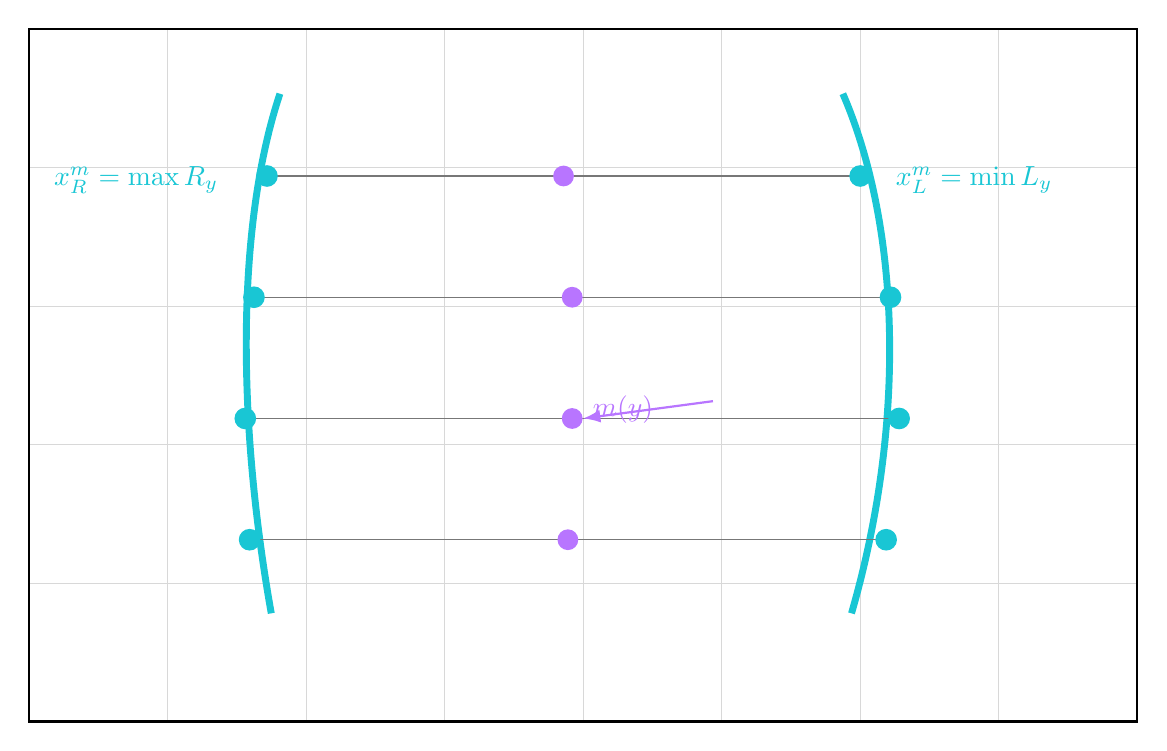
\begin{tikzpicture}[x=0.055cm,y=0.055cm]
    \draw[step=32, gridgray, very thin] (0,0) grid (256,160);
    \draw[black, thick] (0,0) rectangle (256,160);

    \draw[maskcyan, line width=2.5pt] (56,25) .. controls (48,70) and (48,115) .. (58,145);
    \draw[maskcyan, line width=2.5pt] (190,25) .. controls (203,70) and (201,115) .. (188,145);

    \foreach \y/\xl/\xr in {42/51/198,70/50/201,98/52/199,126/55/192} {
        \draw[helpergray, thin] (\xr,\y) -- (\xl,\y);
        \fill[maskcyan] (\xl,\y) circle (2.5);
        \fill[maskcyan] (\xr,\y) circle (2.5);
        \fill[axispurple] ({(\xl+\xr)/2},\y) circle (2.4);
    }

    \node[maskcyan, anchor=east] at (46,125) {\(x_R^m=\max R_y\)};
    \node[maskcyan, anchor=west] at (198,125) {\(x_L^m=\min L_y\)};
    \node[axispurple, anchor=west] at (128,72) {\(m(y)\)};
    \draw[-{Latex[length=2.2mm]}, axispurple, thick] (158,74) -- (128,70);
\end{tikzpicture}
\caption{Each accepted row contributes the midpoint between the two medial
contour edges. The same rule is used for the pelvic outlet pair and the pubic
symphysis pair.}
\end{figure}

\section*{Step 2: Fit the Medial Axis}

The sample points \(S\) are fit with a straight line using principal component
analysis. In implementation, this is done with singular value decomposition.

\[
    o = \frac{1}{|S|}\sum_{s_i \in S} s_i
\]

The centered sample matrix \(C\) contains rows \(s_i - o\). The first right
singular vector of \(C\) is the unit axis direction \(d\). The direction is
flipped if needed so that \(d_y \ge 0\), giving a stable top-to-bottom axis.

For each sample:

\[
    t_i = (s_i - o) \cdot d
\]

The visualized axis segment spans from:

\[
    o + d\min_i(t_i)
    \quad \textrm{to} \quad
    o + d\max_i(t_i)
\]

\section*{Step 3: Place the POD Cross-Line}

The lateral pelvic outlet points are projected onto the medial axis:

\[
    t_L = (p_L - o)\cdot d,
    \qquad
    t_R = (p_R - o)\cdot d
\]

where \(p_L\) is \texttt{L-LPO} and \(p_R\) is \texttt{R-LPO}, both represented
in the 512 by 512 mask coordinate system. The POD center is halfway between
those two projected locations, clamped to the fitted sample extent:

\[
    t_{mid} =
    \operatorname{clamp}
    \left(
        \frac{t_L + t_R}{2},
        \min_i(t_i),
        \max_i(t_i)
    \right)
\]

\[
    a_{mid} = o + d t_{mid}
\]

The POD direction is perpendicular to the fitted medial axis:

\[
    n = (-d_y, d_x)
\]

Starting from \(a_{mid}\), the application searches each pelvic outlet contour
for an endpoint on the appropriate side of this normal. It searches in expanding
bands around the perpendicular cross-section and picks the outward-most contour
pixel for each side. The returned \texttt{POD} annotation is the line segment
between those two selected pelvic outlet contour pixels.

\begin{figure}[htbp]
\centering
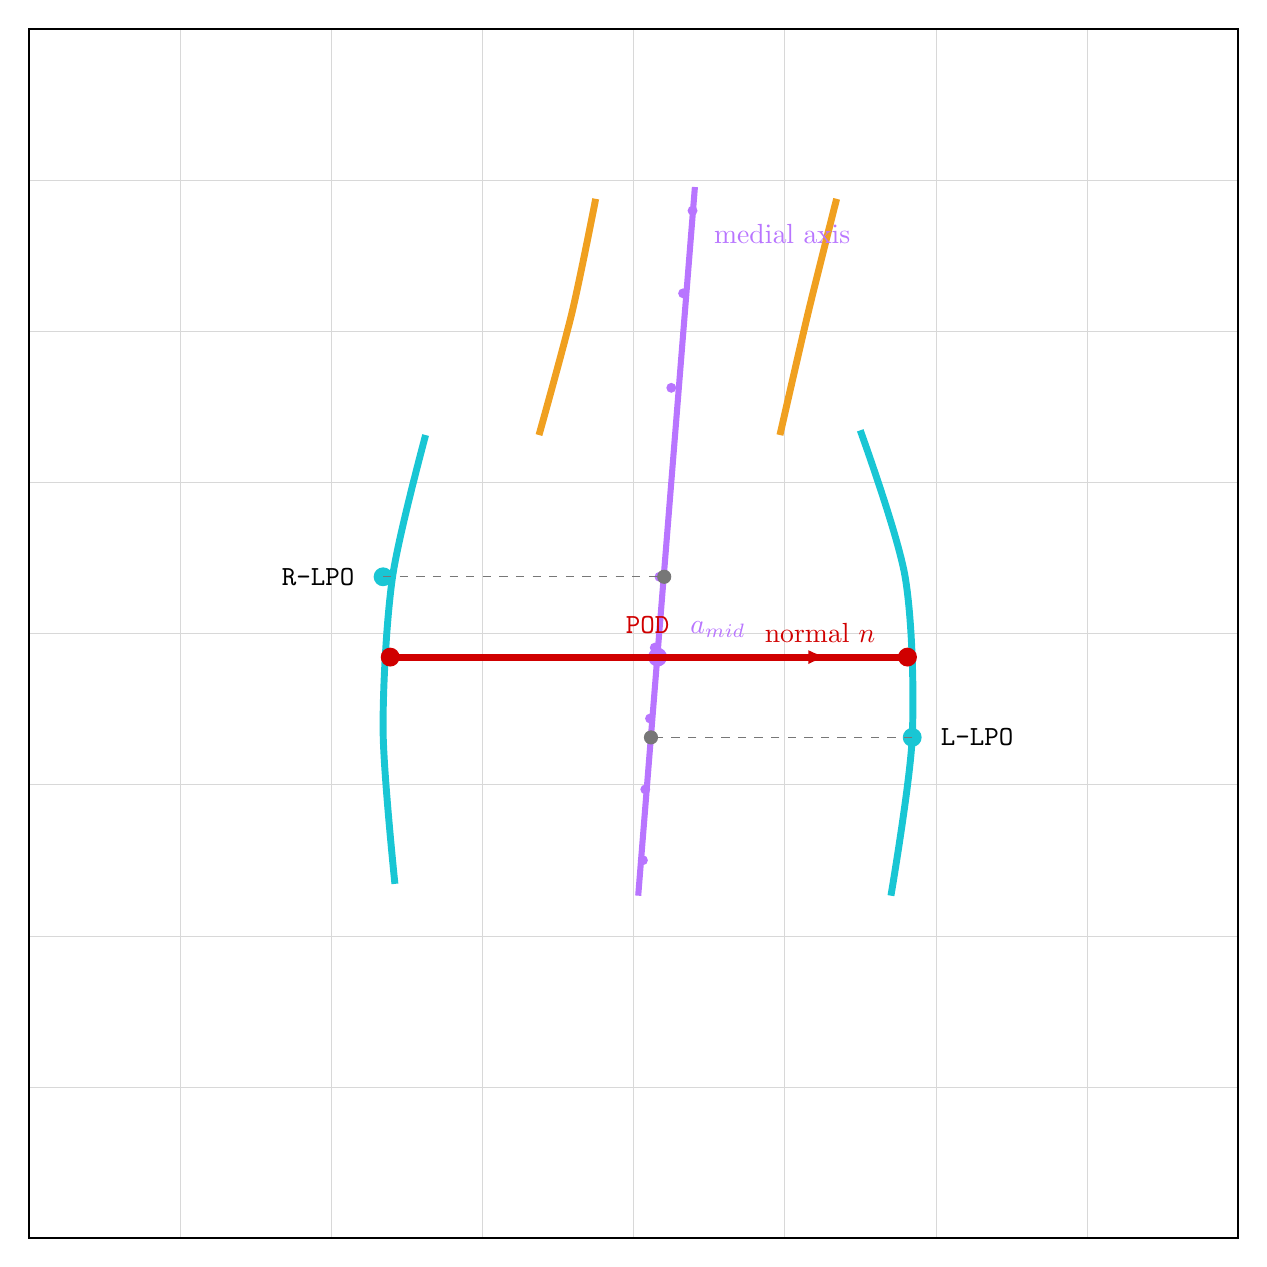
\begin{tikzpicture}[x=0.03cm,y=0.03cm]
    \draw[step=64, gridgray, very thin] (0,0) grid (512,512);
    \draw[black, thick] (0,0) rectangle (512,512);

    \draw[maskcyan, line width=2.5pt] plot[smooth] coordinates
        {(155,150) (150,215) (154,280) (168,340)};
    \draw[maskcyan, line width=2.5pt] plot[smooth] coordinates
        {(365,145) (374,212) (371,280) (352,342)};
    \draw[psorange, line width=2.5pt] plot[smooth] coordinates
        {(216,340) (230,392) (240,440)};
    \draw[psorange, line width=2.5pt] plot[smooth] coordinates
        {(318,340) (330,392) (342,440)};

    \foreach \p in {(260,160),(261,190),(263,220),(265,250),(267,280),(272,360),(277,400),(281,435)} {
        \fill[axispurple] \p circle (2.1);
    }

    \draw[axispurple, line width=2.2pt] (258,145) -- (282,445);
    \node[axispurple, anchor=west] at (286,425) {medial axis};

    \coordinate (LLPO) at (374,212);
    \coordinate (RLPO) at (150,280);
    \coordinate (LPROJ) at (263.4,212);
    \coordinate (RPROJ) at (269,280);
    \coordinate (MID) at (266.2,246);
    \coordinate (LPOD) at (372,246);
    \coordinate (RPOD) at (153,246);

    \fill[maskcyan] (LLPO) circle (4);
    \fill[maskcyan] (RLPO) circle (4);
    \node[anchor=west] at (382,212) {\texttt{L-LPO}};
    \node[anchor=east] at (142,280) {\texttt{R-LPO}};

    \draw[helpergray, dashed] (LLPO) -- (LPROJ);
    \draw[helpergray, dashed] (RLPO) -- (RPROJ);
    \fill[helpergray] (LPROJ) circle (3);
    \fill[helpergray] (RPROJ) circle (3);

    \fill[axispurple] (MID) circle (4);
    \node[axispurple, anchor=south west] at (276,250) {\(a_{mid}\)};

    \draw[podred, line width=2.5pt] (RPOD) -- (LPOD);
    \fill[podred] (LPOD) circle (4);
    \fill[podred] (RPOD) circle (4);
    \node[podred, anchor=south] at (262,252) {\texttt{POD}};

    \draw[-{Latex[length=2.4mm]}, podred, thick] (MID) -- (338,246);
    \node[podred, anchor=south] at (335,248) {normal \(n\)};
\end{tikzpicture}
\caption{The LPO points are projected onto the medial axis. The halfway point
between those projections defines the cross-section. The final POD line is the
perpendicular segment from the right pelvic outlet contour to the left pelvic
outlet contour.}
\end{figure}

\section*{Effect of the Pubic Symphysis Contours}

Before the latest change, the medial axis was fit only from
\texttt{L-C-PO}/\texttt{R-C-PO}. Now, when \texttt{L-C-PS} and \texttt{R-C-PS}
are both annotated, their row-wise midpoint samples are added to the same fit.
This lets the lower pelvic midline influence the axis, which is useful when the
two outlet contours alone produce a centerline that is visually offset from the
overall bilateral symmetry.

The PS contours do not replace the outlet contours. The endpoint search for the
POD line still uses \texttt{L-C-PO} and \texttt{R-C-PO}; the PS contours only
improve the fitted medial axis used to choose the POD cross-section and angle.

\section*{Failure Cases}

The application does not generate a POD line when:

\begin{itemize}
    \raggedright
    \item either pelvic outlet contour mask is missing or empty;
    \item either lateral pelvic outlet point is unavailable;
    \item the PO and optional PS contour pairs do not produce at least two valid
    midpoint samples in total;
    \item the SVD line fit is degenerate;
    \item a POD endpoint cannot be selected from either pelvic outlet contour.
\end{itemize}

\section*{Implementation Location}

The current implementation is in \texttt{app/src/main.py}:

\begin{itemize}
    \item \texttt{\_protocol\_pod\_medial\_axis\_samples}: builds row-wise
    midpoint samples for one left/right contour pair;
    \item \texttt{\_fit\_protocol\_pod\_medial\_axis}: fits the straight medial
    axis using SVD;
    \item \texttt{\_protocol\_pod\_perpendicular\_endpoint}: chooses the PO
    contour endpoint for one side of the POD line;
    \item \texttt{\_derive\_protocol\_pod}: combines PO and optional PS samples
    and returns the final POD segment.
\end{itemize}

\end{document}
